\subsection{Problem Definition}
\label{sec:problem}

%\section{Approach}
%\label{sec:approach}
%
%\subsection{Preliminaries}
%\label{subsec:preliminaries}
Next, we introduce notation and definitions used in our approach, and we formally define the problem addressed in this paper.

%present necessary formal definitions, we describe how the distance between two geolocated time series is computed, and then we formally define the problem addressed in this paper.

A {\em time series} is a time-ordered sequence of values $T = \{v_1, \ldots, \\v_w\}$, where $v_i$ is the value at the $i$-th time point and $w$ is the length of the series. In particular, we deal with time series that are additionally characterized by a \emph{location}, denoted by $T.loc$. Assuming a 2-dimensional space, we further use the notation $T.loc_x$, $T.loc_y$ to refer to the $(x,y)$ coordinates of $T$'s location. 

In the {\em spatial domain}, the distance between two geolocated time series $T$ and $T'$ of equal length $w$ is calculated using the Euclidean distance of their respective locations. Furthermore, we normalize this distance with $maxDist_{sp}$, i.e., the maximum spatial distance of any pair of objects in the dataset, to obtain a measure in the interval $[0,1]$. Thus:
\begin{equation} \label{eq:dist_sp}
dist_{sp}(T, T') = \frac{\sqrt{(T.loc_x - T'.loc_x)^2 + (T.loc_y - T'.loc_y)^2}}{maxDist_{sp}}
\end{equation} \label{eq:2}

%\vspace{-5pt}
In the {\em time series domain}, similarly to other prior works (e.g., \cite{shieh2008kdd}), we also apply the Euclidean distance to measure the similarity of a pair of objects. In future work, we plan to make use of more complex distance measures \cite{paparrizos2015k}. More specifically, we calculate the distance between two time series $T$ and $T'$ as follows:
\begin{equation} \label{eq:dist_ts}
dist_{ts}(T, T') = \frac{\sqrt{\displaystyle \sum_{i=1}^{w}(v_i - v'_i)^2}}{maxDist_{ts}}
\end{equation}

%\vspace{-5pt}
\noindent where $maxDist_{ts}$ denotes the maximum distance of any pair of objects in the dataset and is used for normalization, as above.

To index and summarize time series, we use the notion of {\em Minimum Bounding Time Series} (MBTS). An MBTS is a summarization of a set of time series $\mathcal{T}$, defined by a pair of upper and lower time series bounds that contain them. Formally, given a set of time series $\mathcal{T}$, its MBTS consists of an \emph{upper bounding time series} $T_{up}$ and a \emph{lower bounding time series} $T_{lo}$, constructed by selecting the maximum (for $T_{up}$) and minimum (for $T_{lo}$) of values at each time point among all time series of the set as follows:

%\vspace{-3pt}
\begin{align}\label{eq:bounds1}
 \begin{split}
  & T_{up} = \{ \max_{T \in \mathcal{T}} T[0], \ldots, \max_{T \in \mathcal{T}} T[w-1] \} \\
  & T_{lo} = \{ \min_{T \in \mathcal{T}} T[0], \ldots, \min_{T \in \mathcal{T}} T[w-1] \}
 \end{split}
\end{align}



%We use the term \emph{geolocated time series} (GTS) to reference to time series associated with a location. 

%\btsr employs the following {\em distance measures} for similarity search on geolocated time series.



% Based on the above, we derive a {\em hybrid distance} measure $dist_h(T, T')$ between two geolocated time series $T$ and $T'$, combining both their distances $dist_{sp}(T, T')$ in the spatial domain and $dist_{ts}(T, T')$ in the time series domain. For that purpose, an {\em exponential decay} function is applied to decrease the similarity of two time series based on their spatial distance:
% \begin{equation}
%  sim_h(T, T') = sim_{ts}(T, T') \; e^{- \gamma \; dist_{sp}(T, T')}
%  \label{eq:sim_h}
% \end{equation}

% \noindent where $sim_{ts}(T, T') = 1 - dist_{ts}(T, T')$ and $\gamma$ is the exponential decay constant. Then:
% \begin{equation}
%  dist_h(T, T') = 1 - sim_h(T, T')
%  \label{eq:dist_h}
% \end{equation}

% Accordingly, the hybrid similarity (distance) between two geolocated time series $T$ and $T'$ is equal to their standard time series similarity (distance) if they are located at the same position, and it gradually decreases (respectively, increases) if one is placed farther apart from the other.

We can now formally introduce our problem. Given a set of geolocated time series and an area, our goal is to produce a summary for visualization comprising the following two parts: 

%	\vspace{3pt}
\begin{itemize}
	\item \emph{Time series summary}: A collection of MBTSs (\emph{bundles}), summarizing the time series located within the given area.
%	\vspace{2pt}
	\item \emph{Spatial summary}: A set of MBRs, each one associated with an object counter for each identified bundle.
\end{itemize}
%	\vspace{3pt}
	
The bundles provide a summarization of the time series that are contained within their MBTSs. Figure~\ref{fig:example_bundle} depicts an example of two time series bundles for two different sets of time series. Regarding the spatial summary, for each MBR associated with a certain bundle, the counter denotes the number of time series contained in it.

\begin{figure}[!ht]
	\centering
	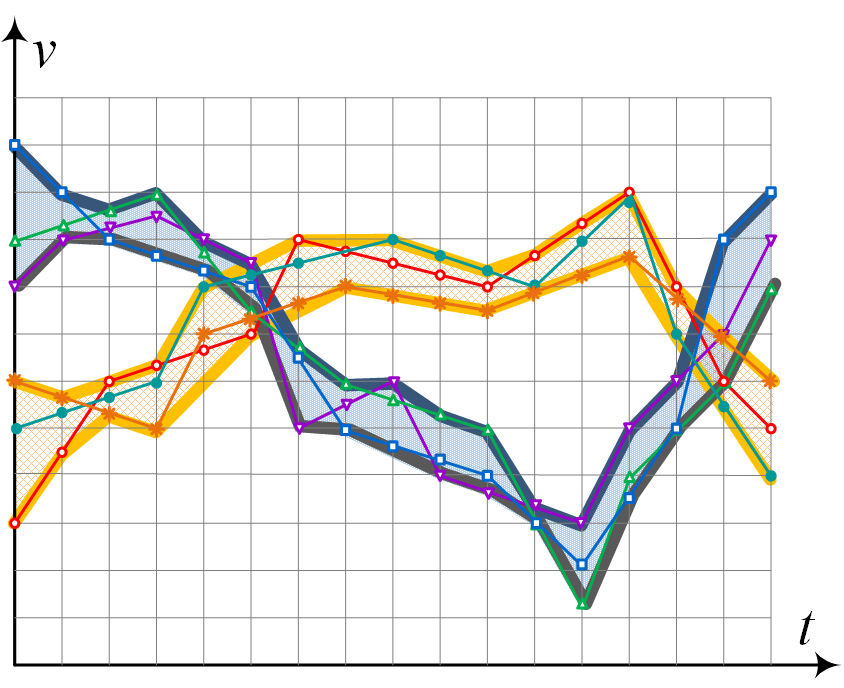
\includegraphics[width=0.8\columnwidth]{figures/bounds_ctsr.png}
	%\vspace{-5pt}
	\caption{Example illustrating the resulting bundles for two sets of time series.}
	%\vspace{-5pt}
	\label{fig:example_bundle}
\end{figure}


\subsection{Approach}
\label{sec:approach}

We propose a visualization method for geolocated time series that draws on a map the time series and spatial summaries for the current visible area. Using this process, a user can select the bundle of her preference and the proper spatial summary will appear on the map after acquiring the necessary MBRs from the \btsr index. Whenever the user zooms in/out or moves around the map, the \btsr is traversed, and the corresponding bundles, MBRs and object counts are obtained to drive the visualization. In each case, the rectangle corresponding to the visible part of the map is used to feed a traversal algorithm that efficiently gathers the results. In the following, we describe this process in detail, after providing some necessary background information on the \btsr index.

\subsubsection{The \btsr Index}
\label{subsec:btsr}

To efficiently generate real-time visualizations of geolocated time series data, we need early access to both spatial and time series related information while traversing the index, in order to maintain low latency levels when drawing the required graphic elements. However, none of the approaches presented in Section~\ref{sec:related} supports geolocated time series indexing. To the best of our knowledge, the recently proposed \btsr index \cite{chatzig17btsr} is the only one that provides the desired functionality. 

The \btsr is based on the R-tree \cite{Guttman1984} for the spatial indexing part. The R-tree organizes a hierarchy of nested $d$-dimensional rectangles. Each node corresponds to a disk page and represents the MBR of its children or, for leaf nodes, the MBR of its contained geometries. The number of entries per node (excluding the root) is between a lower bound $m$ and a maximum capacity $M$. Query execution in R-trees starts from the root. MBRs in any visited node are tested for intersection against the search region. Qualifying entries are recursively visited until the leaf level or until no further overlaps are found. Several paths may be probed, as multiple sibling entries could overlap with the search region. The \btsr extends the information stored within each node of the R-Tree with bundles of MBTSs. This allows to efficiently prune the search space when evaluating hybrid queries combining time series similarity with spatial proximity.

%\snote{[I don't think we need to introduce the various queries here. Only the structure of the index is relevant.]}


%\subsection{The \btsr Index}
%\label{subsec:btsr_tree}

%\snote{[Remove: }
% \subsubsection{Hybrid Queries}
% \label{subsubsec:h_queries}
% \btsr supports {\em hybrid queries} on geolocated time series, i.e., queries that retrieve search results based on both spatial distance and time series distance. In these queries, a geolocated time series $T_q$ is given as a reference, and the goal is to identify similar time series to $T_q$, based on both spatial distance and time series distance. \btsr supports the following hybrid queries:

% \begin{itemize}
%  \item $Q_{bb}(T_q, \theta_{sp}, \theta_{ts})$. This query applies two individual boolean filters. It retrieves each time series $T$ having $dist_{sp}(T_q, T) \leq \theta_{sp}$ and $dist_{ts}(T_q, T) \leq \theta_{ts}$. In other words, it retrieves all time series that are located within a radius $\theta_{sp} \cdot maxDist_{sp}$ from $T_q$'s location and their time series dissimilarity to $T_q$ is at most $\theta_{ts} \cdot maxDist_{ts}$.
%  \item $Q_{kb}(T_q, k, \theta_{ts})$. This query retrieves the $k$ time series closest to $T_q$'s location also having $dist_{ts}(T_q, T) \leq \theta_{ts}$.
%  \item $Q_{bk}(T_q, \theta_{sp}, k)$. This query retrieves the $k$ most similar time series to $T_q$ which are also located within distance $\theta_{sp} \cdot maxDist_{sp}$ from $T_q$'s location.
%  \item $Q_{hb}(T_q, \theta_h, \gamma)$. This query retrieves all time series having hybrid distance to $T_q$ at most $\theta_h$, i.e., $dist_h(T_q, T) \leq \theta_h$.
%  \item $Q_{hk}(T_q, k, \gamma)$. This query retrieves the $k$ time series with the smallest hybrid distance $dist_h(T_q, T)$ to $T_q$.
% \end{itemize}

%\snote{]}

As in the standard R-tree, each node of the \btsr has at least $m$ and at most $M$ entries and stores the MBRs of its children. Additionally, for each child, a node stores a pre-specified number of time series bundles, each consisted of an MBTS that encloses all the time series indexed in its subtree. Each bundle is calculated using Equation \ref{eq:bounds1}. Construction and maintenance of the \btsr follow the procedures of the R-tree for data insertion, deletion and node splitting. Objects (i.e., geolocated time series) are inserted into leaf nodes, and any resulting changes are propagated upwards. Once the nodes have been populated, the bundles of each node are calculated bottom-up. To construct the time series bundles within each node, we rely on $k$-{\em means clustering}. The objects contained in each node are clustered according to their Euclidean distance on the time series domain. The example in Figure \ref{fig:example_bundle} depicts the bundles (the two bands with a thick outline) obtained for a set of time series (shown as thin polylines) when the number of clusters is set to $k=2$.

%Similarly to \ref{eq:bounds1}, let $\mathcal{T}_N$ denote the set of objects contained in the subtree rooted at entry $N$ of a node. Then, for each bundle of $N$, the MBTS comprises two (virtual) time series, $T_{N,up}$ and $T_{N,lo}$, which are derived by selecting the maximum and minimum values, respectively, among all the time series within that specific bundle, i.e.:

% \begin{align}\label{eq:bounds2}
%  \begin{split}
%   & T_{N,up} = \{ \max_{T \in \mathcal{T}_N} T[0], \ldots, \max_{T \in \mathcal{T}_N} T[w-1] \} \\
%   & T_{N,lo} = \{ \min_{T \in \mathcal{T}_N} T[0], \ldots, \min_{T \in \mathcal{T}_N} T[w-1] \}
%  \end{split}
% \end{align}



% \begin{figure}[!ht]
% 	\centering
% 	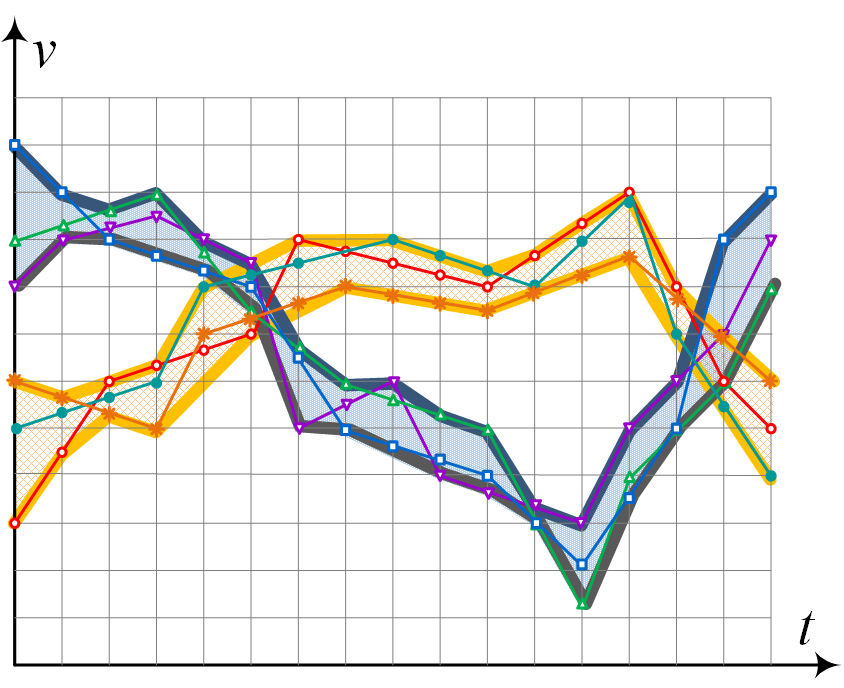
\includegraphics[width=\columnwidth]{figures/bounds_ctsr.png}
% 	\caption{Example illustrating the resulting bundles for a collection of time series.}
% 	\label{fig:example_bundles}
% \end{figure}

%\snote{{\bf CHECK:} If $\beta$ represents the number of clusters obtained from $k$-means, then for  clarity we should better replace symbol $\beta$ with $k$. Moreover, the query rectangle could be simply denoted as $q$ and the number of requested bundles as $k$.}

%In the following, we use $\beta$ to refer to the number of bundles to be created in each node. 
For inner nodes, the bundles are constructed bottom-up. First, in each leaf node, the contained time series are clustered into $k$ bundles. Then, the MBTS of each bundle is computed and stored in the node. As a next step, each parent node receives all the MBTSs of its children and computes its own $k$ bundles and respective set of MBTS by clustering them. The process continues upwards, until reaching the root of the tree. Optionally, \emph{Piecewise Aggregate Approximation} \cite{keogh2001paa,faloutsos2000vldb} can be applied over the time series. As detailed in \cite{chatzig17btsr}, this allows a trade off between the number of bundles per node and the MBTS resolution, thus permitting a larger number ($>k$) of bundles in nodes at higher levels in the tree hierarchy.

% \snote{[Tree construction is also not needed:]}

% \paragraph{Tree Construction}
% \label{par:tree}
% The objects are first inserted in the index similarly to R-tree. The heuristic for determining where each object will be inserted can be adapted to also account for the similarity of objects in the time series domain, in addition to their spatial distance. Recall that in the standard R-tree, selecting the node where a new object will be inserted is based on finding the entry where such an insertion incurs the least possible enlargement of its MBR. This is extended to also consider the enlargement incurred in that entry's \emph{absolute} MBTS, which is an overall upper and lower bound for all bundles. More specifically, selecting the appropriate node $N$ should minimize the following hybrid cost function:

% \begin{equation}
%  cost(T, N) = \lambda \cdot cost_{sp}(T, N) + (1 - \lambda) \cdot cost_{ts}(T, N)
%  \label{eq:insertion_cost}
% \end{equation}

% \noindent where $T$ is the new object for insertion, $cost_{sp}$ and $cost_{ts}$ are functions quantifying the cost of enlarging $N$'s MBR and absolute MBTS, respectively, and $\lambda$ is a weight parameter determining the relative importance of the two factors. Notice that for $\lambda = 1$ this heuristic behaves exactly as in the standard R-tree. When checking a given object $T$ for insertion in node $N$, we calculate distance $\delta_i$ between $T$ and current absolute MBTS at each time point $i \in \{ 1, \dots, w \}$:

% \begin{equation}
%  \begin{split}
%   \delta_i = \begin{cases}
% 	T[i] - T_{N, up}[i], & \text{if} \;\; T[i] > T_{N, up}[i] \\
% 	T_{N, lo}[i] - T[i], & \text{if} \;\; T[i] < T_{N, lo}[i] \\
% 	0, & \text{if} \;\; T_{N, lo}[i] \leq T[i] \leq T_{N, up}[i].
% 	  \end{cases}
%  \end{split}
%  \label{eq:delta_ts}
% \end{equation}

% \noindent Such distances $\delta_i$ are shown with dashed red lines in Figure~\ref{subfig:mbts_bounds}. Thus, we can quantify enlargement $cost_{ts} = \sum{\delta_i}$ of MBTS for $N$.

%\snote{I have removed the bottom-up compression as it would not work in our case: the time-series need to be of same length for clustering to work}

In addition, to support the required functionality of our visualization method, we further extend here the information stored in each node with the {\em count} of geolocated time series that are fully contained within each bundle. This is also done bottom-up, while the index is traversed to calculate the bundles. At each leaf node, after the clustering, we propagate the number of members of each cluster to its parent, which, in turn calculates its clusters and aggregates the counts it has received for each bundle's members. This procedure continues up to the root of the tree.


%\subsection{Visual Exploration of Geolocated Time Series}
%\subsection{Summarization of Geolocated Time Series}
\subsubsection{Summary Construction for Map-Based Visualization}
\label{subsec:visualization}

We now present our summarization approach for producing map-based visualizations of geolocated time series. The process is outlined in Algorithm~\ref{alg:algorithm}. It takes as input the {\em query rectangle} ($q$), i.e., the area of the map for which the visualization is produced, and the number of bundles $k$ to be generated. The process comprises three distinct steps. Initially, the \btsr index is traversed to obtain the MBRs contained in the query rectangle, along with their bundles and the number of objects per bundle (Line 1). Next, $k$-means clustering is applied using the average time series per bundle as centroids (Line 2). Finally, the new bundles are calculated and the proper MBRs and corresponding object counts are assigned to each bundle (Line 3). Next, we describe each step in more detail.

%\subsubsection{Step 1: \btsr Traversal}
%\label{subsubsec:traversal}
\emph{Step 1: \btsr Traversal}.
During this step, the \btsr index is traversed, with the target being the fast provision of a predefined number $k$ of geolocated time series bundles contained within the given area $q$, along with the MBRs where these bundles can be found and the total number of geolocated time series that reside within each MBR. All required information is stored within the nodes of the \btsr, thus, when a node that is contained within the query rectangle is found, the relevant information is retrieved and added to the intermediate results, without any need to continue searching in its sub-tree. The output of this step is passed to the next step of the procedure. 

% The $Q_{rb}$ query requires one argument and has the following format:

% \begin{equation}
% Q_{rb}(q)
% \end{equation}

% \noindent where $q$ is the query rectangle, which represents the area on the map where we apply they query.

%Line 1 of Algorithm~\ref{alg:algorithm} initiates the traversal procedure of \btsr index. 

In more detail, the traversal is performed as follows. After initializing a queue with the root's children (Line 7), we loop over it (Line 8) until it's empty. For each inner node's child $N'$, we check whether its MBR is contained within the given query rectangle $q$ (Lines 11--12). If so, its MBR, time series bundles and the number of objects per bundle are added to the intermediate results (Line 13) as a {\em tuple} with the following components:

%\vspace{-2pt}
\begin{equation*}
\langle mbr, \{ (mbts_1,cnt_1), ..., (mbts_k, cnt_k) \} \rangle
\end{equation*}

\noindent Each such tuple indicates the MBR of a node ($mbr$), consisting of the coordinates of the lower left and upper right point, as well as $k$ pairs denoting the bundles of the node along with the corresponding number of objects per bundle. If the MBR is not contained in the query rectangle, we check whether it overlaps with it and if so, we add the child node to the queue (Line 15). If not, this MBR is located outside the query rectangle, and thus we can skip searching this child. Once no more nodes are left to search, the intermediate results are finally returned (Line 16).

%\snote{{\bf CHECK:} For more clarity, symbols like $T_{b,1}$ should be replaced with $mbts_{1}$. These $T$ are not original time series, but pairs of bounds as defined in (\ref{eq:bounds1}), i.e., $MBTS$. Similarly, contents of nodes like $N.b$ should be denoted as $N.mbts$ in analogy to $N.mbr$.}


% \begin{algorithm}[!ht]
% \begin{small}
% 	\DontPrintSemicolon
% 	\KwIn{The query rectangle $q$}
% 	\KwOut{A list $R$ containing tuples}
% 	\Begin{
% 		$R \leftarrow \emptyset$ \\
% 		$L \leftarrow$ root entries \\
% 		\While{$L \neq \emptyset$}{
% 			$N \leftarrow L.getNext()$ \\
% 			\If{$N$ is not leaf}{
% 				\ForEach{$N' \in N.getChildren()$}{
% 					\If{$q.contains(N'.mbr)$}{
% 						$R \leftarrow R \cup \{N'.mbr, N'.b, N'.nObj\}$ \\
% 					}
% 					\ElseIf{$q.overlaps(N'.mbr)$}{
% 						$L \leftarrow L \cup \{N'.getChildren()\}$
% 					}
% 					\Else{
% 						do nothing
% 					}
% 				}
% 			}
% 			\Else{
% 				do nothing
% 			}
% 		}
% 		$return(R)$
% 	}
% 	\caption{$Q_{rb}(q)$}
% 	\label{alg:step1}
% \end{small}		
% \end{algorithm}

%\subsubsection{Step 2: Bundles Clustering}
%\label{subsubsec:clustering}

\emph{Step 2: Bundles Clustering}.
The traversal algorithm returns tuples, each containing the bundles residing in the query rectangle, the corresponding nodes' MBRs and the number of objects per bundle. During step 2, $k$-means clustering is executed on the average time series of each bundle. 

\begin{comment}
The results are then passed to step 3 in order to calculate the final bundles and properly assign the corresponding MBRs.
\end{comment}

%\snote {{\bf CHECK:} Symbol $Tup$ in the pseudocode signifies tuples, but it may be confused with the upper bound of MBTS, as defined in (\ref{eq:bounds1}). Perhaps use a single character like $r$ or $t$?}

Line 2 of Algorithm~\ref{alg:algorithm} calls the clustering procedure. Initially, for each tuple (Line 20), we loop over its bundles (Line 21) and generate a new tuple per bundle of the following format: 

\begin{equation*}
\langle T_{avg}, mbts, cnt, mbr \rangle
\end{equation*}

\noindent This new tuple contains an average time series, the bundle itself ($mbts$), the number $cnt$ of objects enclosed in this bundle, and the MBR ($mbr$) this bundle belongs to (Line 23). The average time series $T_{avg}$ is calculated by averaging the upper and lower bound of each bundle (Line 22), i.e., average value at each time point. The resulting collection of tuples (Line 24) is fed to the $k$-means algorithm in order to return the required number $k$ of bundles to be created. This clustering generates a clustered collection of tuples using the calculated average time series (Line 25). These results are then forwarded to step 3 (Line 26).

% \begin{algorithm}[!ht]
% \begin{small}
% 	\DontPrintSemicolon
% 	\KwIn{The list of tuples $R$ from step 1}
% 	\KwOut{A clustered collection of tuples $R_{c}$}
% 	\Begin{
% 		$R_{c} \leftarrow \emptyset$ \\
% 		$C \leftarrow \emptyset$ \\
% 		\ForEach{$Tup \in R$}{
% 			\ForEach{$b \in Tup.b$}{
% 				$T_{avg} \leftarrow avg(b.up, b.lo)$ \\
% 				$Tup' \leftarrow \{T_{avg}, b, Tup.nObj(b), Tup.mbr\}$ \\
% 				$C \leftarrow C \cup Tup'$ \\
% 			}
% 		}
% 		$R_{c} \leftarrow kmeans(C.avg)$ \\
% 		$return(R_{c})$
% 	}
% 	\caption{$BundlesClustering(R)$}
% 	\label{alg:step2}
% \end{small}		
% \end{algorithm}

%\subsubsection{Step 3: Bundles Calculation and MBR Assignment}
%\label{subsubsec:assignment}

\emph{Step 3: Bundles Calculation and MBR Assignment}.
During step 3, the clustered tuples received from step 2 are used to calculate the final bundles, corresponding MBRs and total number of objects per MBR are assigned to each bundle. The final bundles are calculated in a similar manner to the MBTS bundles during \btsr construction. More specifically, at each time point, we obtain the maximum and minimum value among the corresponding upper and lower bounds for the bundles of each cluster (see Section \ref{subsec:btsr}). In case two MBRs that belong to the same final bundle are the same, their number of objects is aggregated. The final result is then forwarded to the visualization layer.
%our visualization method, which will be presented in the next section.


%\snote{{\bf CHECK:} Perhaps, routine $updateBundle$ in Line 33 should be called $updateMBTS$ for consistency with the rest.}

Line 3 of Algorithm~\ref{alg:algorithm} calls the corresponding procedure. For each cluster of tuples received from step 2 (Line 29), we loop over its members (Line 32) and we use each tuple's bundle and MBR to update the upper and lower bounds and the collection of MBRs that are contained in the final bundle (Lines 33--34). Once the bounds and the corresponding list of MBRs for the current bundle have been calculated, we issue an aggregated tuple to the final result (Line 35). This tuple has the following components:

\begin{equation*}
\langle mbts', \{ (mbr_1,cnt_1), ..., (mbr_n, cnt_n) \} \rangle
\end{equation*}

%\snote{{\bf CHECK:} Alternative notation to stress correspondence of MBRs with counts; also note that $T'_b$ is replaced by $mbts$: \\
%$\langle mbts, \{ (mbr_1,cnt_1), ..., (mbr_n, cnt_n) \} \rangle$ }

\noindent where $mbts'$ is a resulting bundle, along with the MBRs associated with it. Note that the number $n$ of MBRs (as well as their shape) may be varying per bundle, reflecting the spatial distribution of the respective pattern. Each MBR is accompanied with the corresponding number of objects (i.e., raw time series) therein. The final result with all such tuples is then returned in order to generate the visualization (Line 36).

% \begin{algorithm}[!ht]
% \begin{small}
% 	\DontPrintSemicolon
% 	\KwIn{The list of clustered tuples $R_{c}$ from step 2}
% 	\KwOut{A list $R_{f}$ containing the final tuples}
% 	\Begin{
% 		$R_{f} \leftarrow \emptyset$ \\
% 		\ForEach{$Cl \in R_{c}.clusters$}{
% 			$B \leftarrow \emptyset$ \\
% 			$M \leftarrow \emptyset$ \\
% 			\ForEach{$Tup \in Cl$}{
% 				$B \leftarrow updateBundle(B, Tup.b)$ \\
% 				$M \leftarrow updateMBRs(M, Tup.mbr, Tup.nObj)$ \\
% 			}
% 			$R_{f} \leftarrow R_{f} \cup \{B, M\}$ \\
% 		}
% 		$return(R_{f})$
% 	}
% 	\caption{$BundlesMBR(R_{c})$}
% 	\label{alg:step3}
% \end{small}		
% \end{algorithm}


\begin{algorithm}[!t]
	\DontPrintSemicolon
	\KwIn{The query rectangle $q$; the number of bundles to be generated $k$}
	\KwOut{A list $R$ containing tuples of bundles, MBRs and object counts}
%	\tcc{Step 1}
	$R \leftarrow IndexTraversal(q)$   \tcp*{Step 1}
%	\tcc{Step 2}
	$R_{c} \leftarrow BundlesClustering(R, k)$   \tcp*{Step 2}
%	\tcc{Step 3}
	$R_{f} \leftarrow BundlesCalculation(R_{c})$   \tcp*{Step 3}
	\KwRet $R_{f}$ \\
	\vspace{6pt}
	\SetKwProg{procTraversal}{Procedure}{}{}
	\procTraversal{$IndexTraversal(q)$}{
		$R \leftarrow \emptyset$ \\
		$Q \leftarrow Root.getChildren()$ \\
		\While{$Q \neq \emptyset$}{
			$N \leftarrow Q.getNext()$ \\
			\If{$N$ is not leaf}{
				\ForEach{$N' \in N.getChildren()$}{
					\If{$q.contains(N'.mbr)$}{
						\mbox{$R \leftarrow R \cup \{\langle N'.mbr, \{N'.mbts\}, \{N'.cnt\} \rangle\}$} \\
					}
					\ElseIf{$q.overlaps(N'.mbr)$}{
						$Q \leftarrow Q \cup N'.getChildren()$
					}
				}
			}
		}
		\KwRet $R$ \\
	}
	\vspace{6pt}
	\SetKwProg{procCluster}{Procedure}{}{}
	\procCluster{$BundlesClustering(R, k)$}{
		$R_{c} \leftarrow \emptyset$ \\
		$C \leftarrow \emptyset$ \\
		\ForEach{$t \in R$}{
			\ForEach{$b \in t.mbts$}{
				$T_{avg} \leftarrow avg(b.up, b.lo)$ \\
				$t' \leftarrow \langle T_{avg}, b, t.cnt(b), t.mbr \rangle$ \\
				$C \leftarrow C \cup \{ t' \} $ \\
			}
		}
		$R_{c} \leftarrow kmeans(C.avg, k)$ \\
		\KwRet $R_{c}$
	}
	\vspace{6pt}
	\SetKwProg{procBundles}{Procedure}{}{}
	\procBundles{$BundlesCalculation(R_{c})$}{
		$R_{f} \leftarrow \emptyset$ \\
		\ForEach{$Cl \in R_{c}.clusters$}{
			$B \leftarrow \emptyset$ \\
			$M \leftarrow \emptyset$ \\
			\ForEach{$t \in Cl$}{
				$B \leftarrow updateMBTS(B, t.mbts)$ \\
				$M \leftarrow updateMBRs(M, t.mbr, t.cnt)$ \\
			}
			$R_{f} \leftarrow R_{f} \cup \{ \langle \{B\}, \{M\} \rangle \} $ \\
		}
		\KwRet $R_{f}$
	}
	\caption{Summarization of Geolocated Time Series}
	\label{alg:algorithm}
\end{algorithm}